\label{heap}
%\section{Description}

Heapsort is an in-place sort which works in $O(NlogN)$ time in the average and
worst case. It begins by creating a structure known as a \n{heap}, a binary tree
in which a parent is always larger its child, and the largest key is at the top
of the heap. It then repeatedly removes the largest key from the top and places
it in its final position in the array, fixing the heap as it goes.

\subsection{Implicit Heaps}

A \n{binary tree} is a linked data structure where a node contains data and links
to two other nodes, which have the same structure. The first node is called the
\n{parent}, while the linked nodes are called \n{children}. One node is called the
\n{root}, and the tree branches out from this, with each level having twice as many
nodes as the previous level.

A heap is a type of binary tree with several important properties. Firstly, the
the data stored by the parent must always be greater than the data stored by its
children. Secondly, in a binary tree there is no requirement that the tree be full.
In a heap, it is important that every node's left child exists before its right
child. With this property, a heap can be stored in an array without any wasted
space, and the links are implied by a nodes position, rather than by a pointer
or reference. A heap done in the fashion is called an \n{implicit heap}.

To take advantage of the heap structure, it must be possible to easily traverse
the heap, going between parent and child, without the presence of links. This
can be done due to the nature of the indices of parents and their children. In
the case of an array indexed between $0$ and $N-1$, a parent whose index is
$i$ has two children with indices of $2i+1$ and $2i+2$. Conversely, the index of
a parent whose child has an index of $j$ is $\lfloor{}(j+1)/2-1\rfloor{}$. It is
also possible to index the array between $1$ and $N$, in which case the children
have indices of $2i$ and $2i+1$, while the parent has an index of
$\lfloor{}j/2\rfloor{}$. Using this scheme can reduces instruction cost, but
results is slightly more difficult pointer arithmetic, which cannot be performed
in some languages\footnote{In C this can be done by \cc{Item a[] =
\&array[-1];}}.

\subsection{Sorting with Heaps}
To sort an array with a heap, it is necessary to first create the heap. This is
known as \n{heapifying}, and can be performed in two ways.

The first method involves \n{sifting}\footnote{Sifting up and down is also
referred to as fixing up and down, and algorithms that do this are called
\n{fix-up} or \n{sift-up}, and \n{fix-down} or \n{sift-down}.} keys up the heap.
Assuming that a heap already exists, adding a key and re-heapifying will
maintain the heap property. This can be done by adding the key at the end of
the heap, then moving the key up the tree, swapping it with smaller parents
until it is in place. An unsorted array can be sorted by continually heapifying
larger lists, thereby implicitly adding one key every time to a sorted heap of
initial size one. This technique was invented by Williams, and LaMarca refers to
it as the \n{Repeated-Adds} algorithm.

The second technique is to heapify from the bottom up, by sifting keys down.
Beginning at half way through the array (this is the largest node with children),
a parent is compared to its two children and swapped down if it is smaller. This
continues upwards until the root of the heap is reached. This is the technique
specified by Floyd and LaMarca refers to this as Floyd's method.

The second step, described next, is to destroy the heap, leaving a sorted array.

\subsubsection{In-place Sorting}
For an in-place sort, a heap is created as specified above. Then the root of the
heap (the largest key) is swapped with the last key in the heap, and the new
root is sifted down the heap which has been shrunk so as not to include the old
root, which is now in its final position. This is repeated for the entire heap,
leaving a fully sorted array.

Floyd suggested an improvement to this, where the new root is sifted straight
down without regard for whether it is larger than its child. Typically, it will
end near the bottom, so sifting up from here should save comparisons. Sedgewick
notes speed improvements only when comparisons are move expensive than swaps,
such as in the case of sorting strings. For integers, this step should not be
done.

\subsubsection{Out-of-place Sorting}
Up until this point, the heap property used has been that a parent will be
larger than its child. If this property is change so that the parent is always
smaller than its child, then the result is an out-of-place sort. The smallest
key is removed from the heap, and placed in its final place in the array. The
heap is then re-heapified. LaMarca refers to the steps involved as
\n{Remove-min}.

\section{Base Heapsort}
LaMarca recommends to use of the Repeated-Adds algorithm for reducing
cache misses. As such, his base heapsort uses Floyd's method, ostensibly at
the behest of major textbooks, each of whom claim Floyd's method gives better
results. This is certainly backed up by Sedgewick, who recommends this method,
but in initial tests, the out-of-place Repeated-Adds technique had a lower
instruction count. Regardless, the base algorithm used here is Floyd's in-place
sort. Code for a base heapsort is in Figure \ref{Simple Base Heapsort}.

\code{Simple Base Heapsort}{base_heapsort.c}

A difficulty of heapsort is the need to do a bounds check every time. In a heap,
every parent must have either no children, or two children. The only exception
to this is the last parent. It is possible that this has only one child, and it
is necessary to check for this as a result. This occurs every two heapifies, as
one key is removed from the heap every step. Therefore it is not possible to just
pretend the heap is slightly smaller, and sift up the final key later, as it
might be with a statically sized heap.

LaMarca overcomes the problem by inserting a maximal key at the end of a heap if
there's an even number of nodes in the array. This gives a second child to the
last element of the heap. This is an effective technique for building the heap,
as the number of keys is static. When destroying the heap, however, the
maximal key must be added to every second operation. This can be avoided
relatively simply with no extra instructions. If the last key in the heap is
left in place as well as being sifted down the heap, it will provide a
sentinel for the sift-down operation. The key from the top of the heap is then
put into place at the end. This technique reduces instruction count by
approximately 10\%.

The only other optimization used is to unroll the loop while destroying the
heap. This has minimal affect, however.

\section{Memory-tuned Heapsort}
\label{memory-tuned heapsort}
LaMarca notes that the Repeated-Adds algorithm has a much lower number of cache
misses than Floyd's. The reason for this is simple. Consider the number of keys 
touched when a new key is added to the heap. In the case of Floyd's method, the
key being heapified is not related to the last key that was heapified. Reuse
only occurs upon reaching a much higher level of the heap. For large heaps, these
keys may be swapped out of the cache by this time. As a result, Floyd's method
has poor temporal locality.

The Repeated-Adds algorithm, however, displays excellent temporal locality. A
key has a 50\% chance of having the same parent, a 75\% of the same grandparent
and so on. The number of instructions, however, increases significantly, and the
sort becomes out-of-place. For this reason, the Repeated-Adds algorithm is used
for memory-tuned heapsort.

The cost of building the heap is completely dominated by the cost of
destroying it. Less than 10\% of heapsort's time is spent building the heap.
Therefore optimizations must be applied when destroying the heap.

LaMarca's first step is to increase spatial locality. When sifting down the
heap, it is necessary to compare the parent with both children. Therefore it is
important that both children reside in the same cache block. If a heap starts at
the start of a cache block, then the sibling of the last child in the cache
block will be in the next cache block.  For a cache block fitting four keys,
this means that half the children will cross cache block boundaries. This can be
avoided by padding the start of the heap. Since the sort is out of place, an
extra cache block can be allocated, and the root of the heap is placed at the end of
the first block. Now, all siblings will reside in the same block.

\begin{figure}[h]
\centering
\subfigure[a normal heap] {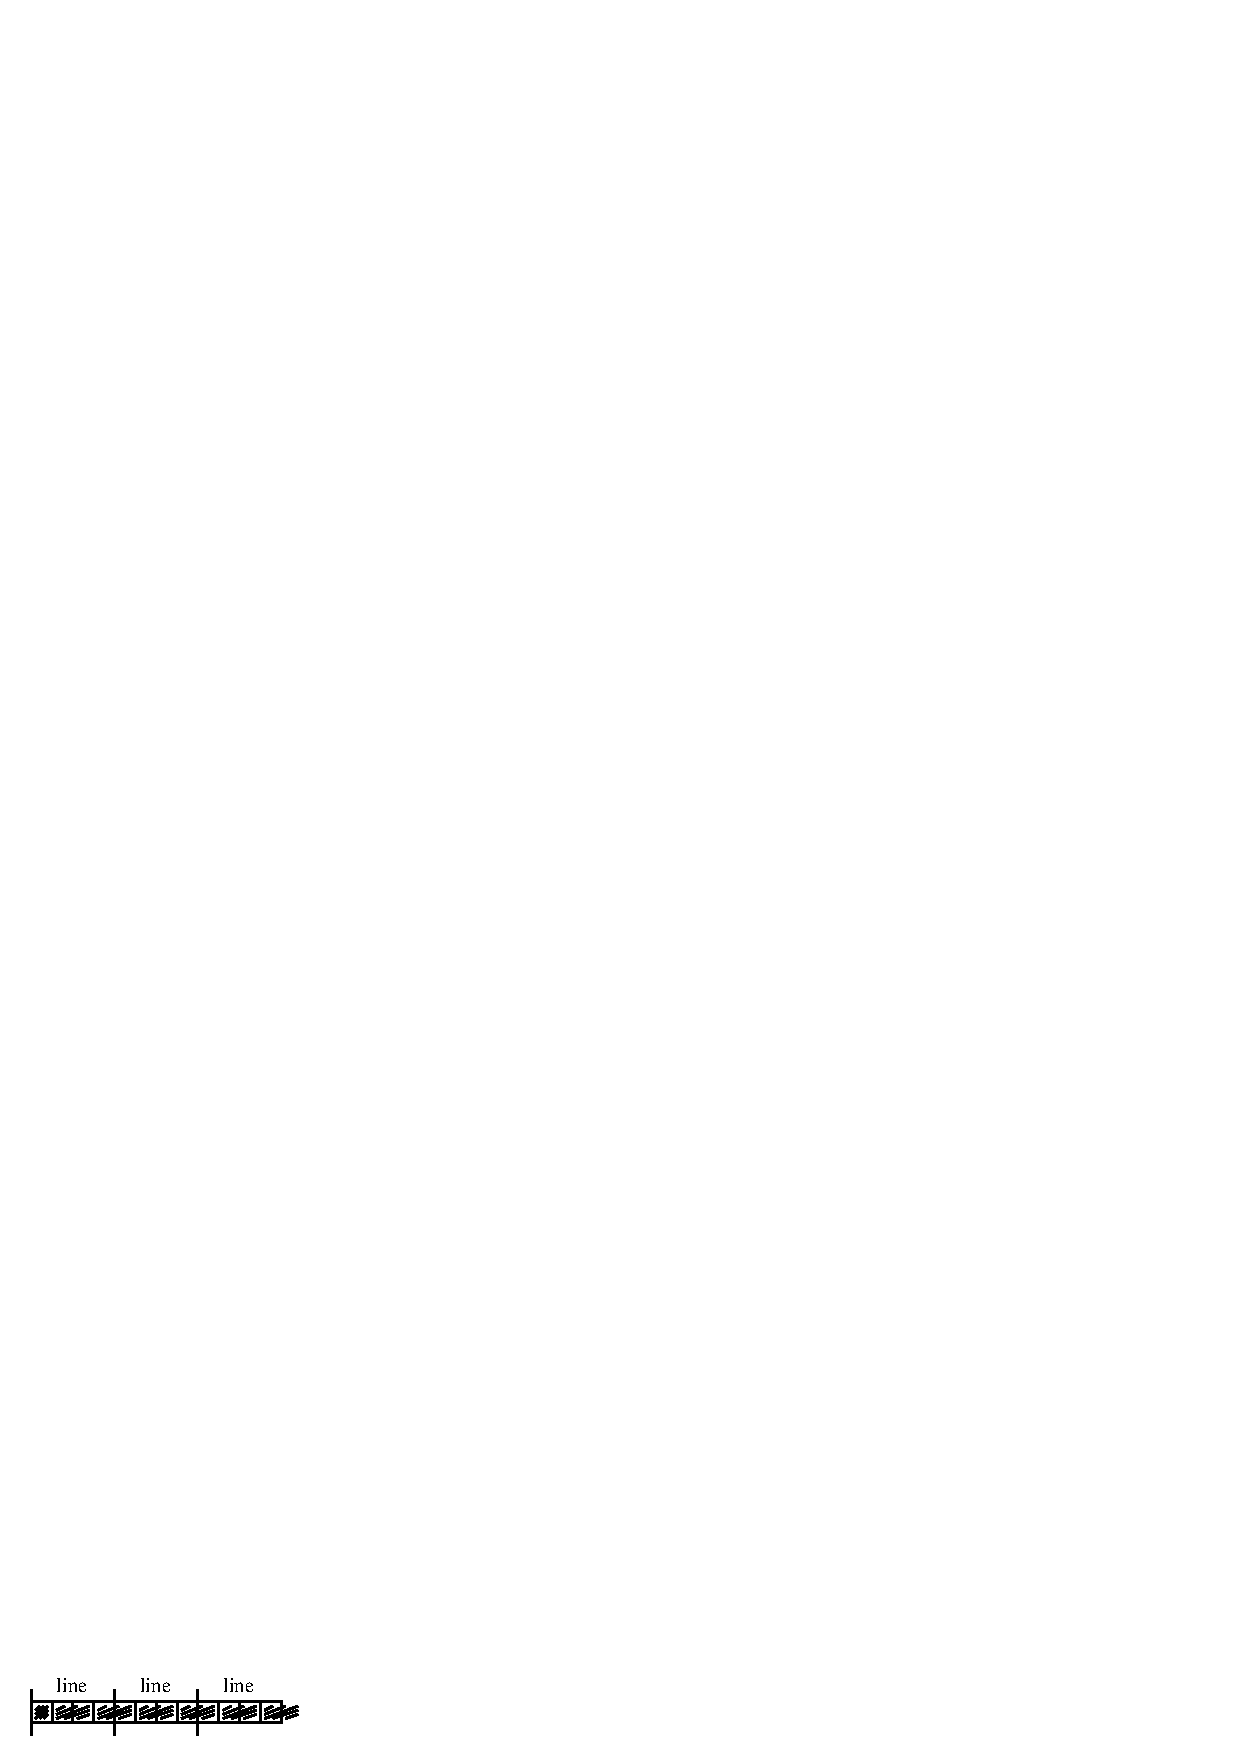
\includegraphics[clip=true]{heap_cache_line1}}
\subfigure[a padded heap] {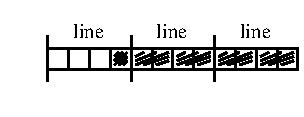
\includegraphics[clip=true]{heap_cache_line2}}
\end{figure}

A second point about heapsort's spatial locality is that when a block is loaded,
only one set of children will be used though two or four sets may be loaded. The
solution is to use a heap higher \n{fanout}, that is, a larger number of
children.  The heap used so far could be described as a 2-heap, since each
parent has two children.  LaMarca proposes using a \n{d-heap}, where $d$ is the
number of keys which fit in a cache line. In this manner, every time a block is
loaded, it is fully used. The number of cache blocks loaded is also decreased,
since the height of the tree is halved by this.

This step changes the indexing formula for the heap. In this method, a parent
$i$ has $d$ children, indexed from $(i*d) + 1$ to $(i*d) + d$. The parent of a
child $j$ is indexed by $\lfloor{}(i-1)/d\rfloor{}$.

The height of a 2-heap is $\lceil{}log_2(N)\rceil{}$, where \textit{N} is the
number of keys in the heap. By changing to a 4-heap, the height is reduced to
$\lceil{}log_4(N)\rceil{} = \lceil{}\tfrac{1}{2}log_2(N)\rceil{}$. The height of
an 8-heap is reduced again to $\lceil{}log_8(N)\rceil{} =
\lceil{}\tfrac{1}{3}log_2(N)\rceil{}$. However, the number of comparisons needed
in each level is doubled, since all the children will be unsorted. LaMarca
claims that as long as the size of the fanout is less than 12, a reduced
instruction count will be observed.

In the base heapsort, an improvement was added that removed the need for a
sentinel. Since the 4- and 8-heaps were unsorted, this optimization had to be
removed. Leaving the key being copied in place was still possible, but it needs
to be replaced by a maximal key before trying to sift the next key down the
heap, lest it were chosen to be sifted up. Placing the sentinel is still cheaper
than the bounds check, however, as the bounds check will need to be performed
$NlogN$ times, compared to $N$ times for the sentinel. The cost of the sentinel
write is more expensive but the extra $logN$ instructions saved will mean that
this increase will be an order of magnitude lower than the bounds check.

\section{Results}
All simulations presented here were performed on 32 byte cache lines. As a
result, 8-heaps were used for heapsort, since 8 4-byte \n{int}s fit the cache line.
LaMarca used 64 bit ints, and while this doesn't affect results, it means that
fewer keys fit into his cache lines. Since modern cache lines are typically
longer than 4 ints, we stick with 32 byte cache lines. \verb!UINT_MAX! was used
as the sentinel.

\subsection{Expected Results}
The instruction count of heapsort is $O(Nlog_d(N))$, although a higher $d$ means
that each step will take longer. As the fanout of the heap doubles, then the
height of the heap halves, but each heap step is more expensive. It is expected
though, that increasing $d$ will reduce the instruction count until the point at
which the cost of a heap step doubles, as compared to a heap with a smaller
fanout.

An additional consideration is that the base heapsort has more instructions than
it's out-of-place equivalent. This means that the 4-heap will have a better
instruction count, as well as better cache performance than the base heapsort.
The 8-heap should have the best cache performance of them all, due to fully
using each cache line, taking advantage of the spatial locality of the cache
line.

LaMarca reports base heapsort has very poor temporal locality, and that the
memory-tuned heapsort will have half the cache misses of base heapsort.

It is expected that the number of comparison branches stays the same with
an increased fanout. When the height of the heap halves, the number of
comparisons in each step doubles. However, the proportion of those which are
predictable changes. The key being sifted down the heap is likely to go the
entire way down the tree. Therefore the comparison between the smallest child
and the parent is predictable. However, the comparisons to decide which child is
smallest are not predictable. In a 2-heap, there is one comparison between
children, meaning that half the branches will probably be correctly predicted.
An 8-heap has seven comparisons between children, and will probably have about
mispredictions, as it behaves similarly to selection sort (See \ref{selection
branches logn}). It is possible, therefore, that the 8-heap will have slightly
fewer mispredictions due to the combination of the shallower heap and the larger
fan-out.

However, the creation of the heap will have fewer misses with a larger fanout,
due to the reduced height. In practice though, the implications of this are
minimal. Most of the time is spent in the destruction of the heap, and this will
have far more branches than the creation phase.

\subsection{Simulation Results}

\plot{heap}{}{}{}{}{}{}

As expected, the 4-heap performs better than the base heapsort. However, the
increased number of comparisons of the 8-heap increases the instruction count to
even higher than base heapsort, due to the disparity between the increase in
comparisons in set of children, and the lesser reduction in the height of the
heap. This is shown in Figure \ref{heap instructions}.

The level 1 cache results, shown in Figure \ref{heap level 1 misses}, show the
difference between the two types of heap. The slope of the base heapsort result
is much greater than all the others, showing base heapsort's poor temporal
locality, with the 8-heap having the fewest misses. This continues into the
level 2 cache, where the flattest slope belongs to the 8-heap. The difference
between fully associative and direct mapped is only minor, with the fully
associative performing slightly better than the direct mapped cache.

In the graph, the base heapsort's results flat-line for a step longer than the
other heapsorts' results. This is due to being in-place, since twice as many
keys fit in the cache without a corresponding increase in misses. For the same
reason, the base heapsorts have no compulsory misses\footnote{See Section
\ref{TODO}.}, while the out-of-place sorts have one compulsory miss in eight,
when the auxiliary heap is being populated.

The branch prediction behaves differently to the expected results, as the
prediction ratio gets worse as the fanout gets larger. The reason we predicted
differently was due to selection sort's $O(log N)$ mispredictions; however, this
is over the entire length of the array, and it is not accurate to extrapolate
these results over a sequence only seven keys long.

The difference between the 4-heap and 8-heap is minor, and the difference for
larger fanout would be less still. The difference between the 2-heap and 4-heap
result is interesting though, the 2-heap has more branches, but less misses per
key.

The difference between different types of predictors is also visible in the
results, shown in Figure \ref{heap branch misses}. The largest table size is
shown for the two-level predictor. The smallest table size is shown for the
bimodal predictor, as all the bimodal table sizes show identical results.  In
the case of the 2- and 8-heaps, the bimodal predictor works better than the
two-level adaptive predictor. The warm-up time of the table-driven predictors is
visible in the base heapsort results, though it's amortised for larger data
sets.

%TODO move this to testing section
Figure \ref{heap cycles} shows the actual time taken for heap sort on a Pentium
4 1.8GHz machine, which has an 8-way associative 256KB level 2 cache with a 64 byte
cache line, a 4-way associative 8KB level 1 data cache, and a maximum branch
misprediction delay of 20 cycles\footnote{This is determined from the Pentium
4's 20 stage pipeline. This number is not exact, and is probably slightly lower,
with the possibility of occasionally rising higher (in the case of an
instruction cache miss, which is exceptionally unlikely for small routines like
sorts).}. Its static branch prediction strategy is backward taken and forward
not taken; its dynamic strategy is unspecified: though \cite{Intel248966-010}
mentions a branch history so it is likely a two-level adaptive predictor.

The figure shows that the base heapsort performs best when the data set fits in
the cache. After that point, the 8-heap performs best, and its cycle count increases
with a smaller slope. This shows the importance of LaMarca's cache-conscious
design even nine years after his thesis. It also shows the importance of reduced
branch mispredictions: the base heapsort has more instructions and level 1 cache
misses, but still outperforms the 4-heap, until level 2 cache misses take over.
However, this is hardly conclusive: the lower level 2 cache misses may account
for this.

The similarities to LaMarca's results are startling. The shape of the
instruction and cache miss curves are identical, as are the ratios between the
base and memory-tuned versions in the case of level 1 and 2 cache misses,
instruction count and execution time.

Slight differences exist though. The level 2 cache miss results here indicate
that while still sorting in the cache, the number of misses in the in-place
heapsort is less than that of the out-of-place sorts. LaMarca, however, has the
same amount of misses in both cases. Similarly, the results here indicate that
base heapsort experiences a sharp increase in cache misses. Memory-tuned
heapsort also has a similar increase, though LaMarca's results show that these
occur at the same position in the graph, in other words, when the set size is
the same. Our results, however, show that this occurs earlier in memory-tuned
heapsort, due to the fact that it is an out of place sort.

Finally, though this is likely to be related the previous differences, base
heapsort performs slightly better for small sets than the memory-tuned heapsort's do in
the results presented here. LaMarca's results indicate that the memory-tuned heapsort
has better results the entire way through the cache. This may relate to the
associativity: LaMarca's tests were performed on a DEC AlphaStation 250 with a
direct mapped cache. The Pentium 4's cache is 8-way associative, and so the
unoptimized algorithm would not suffer as much.

\section{Predictor Results}

\sixplot{base_heapsort_0.eps}{memory_tuned4_heapsort_0.eps}{memory_tuned_heapsort_0.eps}{memory_tuned_heapsort_1.eps}{}{}{base and memory-tuned heapsorts}

The results of the software predictor show the relation of the branches
in the creation and destruction of the heap. The base heapsort results in
Figure \ref{base and memory-tuned heapsorts-1} show that the time taken to
create the heap is not significant relative to the time taken to sort from the
heap.

The most interesting thing is the relation between the predictability of the
comparisons during the destruction of the 2-, 4- and 8-heaps. Compare the
columns marked `\cc{Destruction, child comparison}' and `\cc{Destruction, child
promotion}' in Figure \ref{base and memory-tuned heapsorts-1} (the 2-heap), with
the columns marked `\cc{comparison 1}' to `\cc{child promotion}' in Figure
\ref{base and memory-tuned heapsorts-2} (the 4-heap) and Figures \ref{base and
memory-tuned heapsorts-3} and \ref{base and memory-tuned heapsorts-4} (the
8-heap).

Though the number of times each comparison is used shrinks as the size of the
fanout increased, overall the number of branches increases.  In total, there are
50\% more comparisons in the 4-heap than the 2-heap, and 150\% more in the
8-heap.

More importantly, the accuracy of the each successive comparison increases in
the same way as selection sort (see Section \ref{selection branches logn}),
becoming more predictable as the fanout increases. For example, in the 8-heap,
shown in Figures \ref{base and memory-tuned heapsorts-3} and \ref{base and
memory-tuned heapsorts-4}, the first comparison is predicted correctly 50\% of
the time, while the next is predicted correctly 61\% of the time, then 71\%,
77\%, and so on in a curve, which is shown in Figure \ref{memory-tuned heapsort
curve}.

\begin{figure}
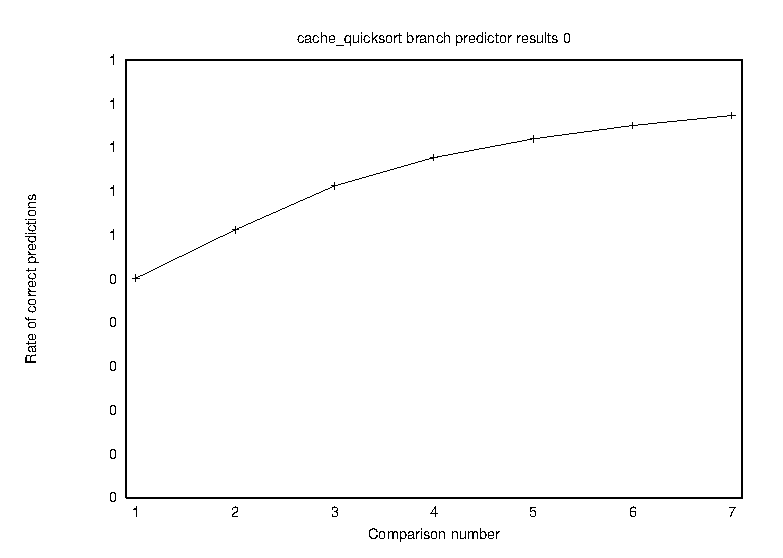
\includegraphics{plots/curve.eps}
\caption{Predictability of branches in memory-tuned heapsort, with a fanout of eight}
\label{memory-tuned heapsort curve}
\end{figure}

\label{heapsort entropy}
We observe here that the more branches there are, the more are correctly
predicted, and that there is a threshold below which the number of branches will
not drop. This is discussed in more Section \ref{quicksort entropy}.

Also notable from the results is that branches are slightly more often not-taken
then they are correctly predicted, implying that a semi-static predictor based
on hints from the compiler could do a better job at making correct predictions.

\section{Future Work}

LaMarca later published heapsort code in \cite{LaMarcaHeap96}. The ACM
Journal of Experimental Algorithms requires that source code be published, and
comparing simulated results from there to the sorts created here might have
interesting results and would explain the discrepancies highlighted in this
chapter.
